\cleardoublepage
\chapter{Softwareengineering}
\label{sec:Kap-1}

Der Bereich des Softwareengineering in der Informatik beschäftigt sich mit der methodischen Entwicklung industrieller Software. 
Softwareengineering verfolgt das (idealisierte) Ziel, möglichst korrekte und zuverlässige Software innerhalb eines bestehenden Zeit- und Kostenrahmens zu erstellen, die die Bedürfnisse aller poten\-tiellen Nutzer bedient. Gleichzeitig soll die Software wartbar und skalierbar sowie in den meisten Fällen auch erweiterbar sein. 

Im Jahr 2018 feierte der Begriff Softwareengineering sein fünfzigjähriges Jubiläum. Eine Konferenz 
\sttpkapitelverweis{NATO-Konferenz Software Engineering}{S.~\pageref{sec:Kap-1.1:NATO-Konferenz}}
mit Experten aus Wissenschaft und Berufsverbänden hatte 1968 erstmalig in einem größeren internationalen Kreis über die Frage diskutiert, wie man Erfahrungen und Methoden aus den Ingenieurwissenschaften für die Entwicklung von Software nutzen könnte. In den folgenden Jahren und Jahrzehnten gab es viele verschiedene Ansätze, den im Rahmen dieser Konferenz international bekannt gewordenen Begriff Softwareengineering mit Leben zu füllen. 

%TODO Maren: Übergang am Ende prüfen
Abschnitt~\ref{sec:Kap-1.1} stellt die Entwicklung des Softwareengineering von seinen Anfängen bis heute dar. Abschnitt~\ref{sec:Kap-1.2} widmet sich anschließend der Frage, was heute unter Softwareengineering verstanden wird und welche Prozesse es beinhaltet. Abschnitt~\ref{sec:Kap-1.3} gibt in Form einer kommentierten Literaturliste einen Überblick über verwendete und weiterführende Literatur für die Themengebiete aus Kapitel~\ref{sec:Kap-1}.

% 1.1
\clearpage
\section{Entwicklung des Softwareengineering}
\label{sec:Kap-1.1}

Bei den ersten Computermodellen der 1940er und 1950er Jahre spielte Software im Vergleich zur Hardware eine stark untergeordnete Rolle. Aufgabe der Software war, die begrenzten – da sehr teuren und aus heutiger Sicht nur wenig leistungsfähigen – Hardwareressourcen, in erster Linie Speicher und Prozessor, optimal auszunutzen. Ein Softwareprogramm der frühen 1950er Jahre setzte sich aus einer Liste von maschinennahen Instruktionen zusammen, die von einer spezifischen Zusammenstellung von Hardwarekomponenten ausgeführt wurden. Softwareentwicklung – der Begriff des Softwareengineering war noch nicht geboren – bedeutete Programmcode zu schreiben, der diese Hardwarekomponenten korrekt und möglichst optimal ansteuerte, auslastete und zusammenarbeiten ließ. Die größte Herausforderung für die Programmierer bestand darin, die Anzahl der Instruktionen möglichst gering zu halten, um ihr Programm im begrenzten Speicherplatz unterzubringen, und effiziente Strategien für die Belegung der oft wenigen Register zu finden.

Programmiert wurde zunächst in \textit{Assemblersprachen}. \marginline{Assembler\-sprachen}
Ein Programm in Assemblersprache wird durch den sogenannten Assemblierer in die Maschinensprache übersetzt. Bei einer reinen Assemblersprache erzeugt dabei jede Anweisung des Assemblercodes genau einen Maschinenbefehl. Eine Assemblersprache ist somit nicht viel mehr als eine lesbarere Darstellung des Binärcodes einer Maschinensprache.  

Seit Mitte der 1950er Jahre wurden die ersten höheren Programmiersprachen\linebreak %%% für Druck
(FORTRAN, Lisp, COBOL, ALGOL) und entsprechende \textit{Übersetzer} 
\marginline{Compiler} 
(engl. Compiler) entwickelt. Ein Übersetzer übersetzt ein Programm, das in einer höheren Programmiersprache geschrieben ist, in Assemblercode oder auch schon direkt in Maschinencode. Die höheren Programmiersprachen und ihre zugehörigen Übersetzer stellten insofern eine Verbesserung dar, als sie die Anwendungsprogrammierer von der Notwendigkeit befreiten, sich mit maschinenabhängigen technischen Details wie begrenzten Befehlsvorräten und der Belegung der Register zu beschäftigen. Sie boten ihnen so die Möglichkeit, sich auf ihr eigentliches algorithmisches Problem zu konzentrieren. 

Bis Ende der 1950er Jahre besaß Software aufgrund der begrenzten hardwaretechnischen Möglichkeiten eine überschaubare Komplexität. Ihre Entwicklung fand meist durch Einzelpersonen oder kleine Teams statt. Mit den Computermodellen der sogenannten dritten Generation, die mit integrierten Schaltungen anstelle von Transistoren arbeiteten und mehrere Programme gleichzeitig im Speicher halten konnten, änderte sich das. Die Leistung der erwerbbaren Hardware verbesserte sich seit Mitte der 1960er Jahre deutlich. Die zunehmende Aufhebung hardwaretechnischer Limitierungen erweiterte aber auch die Menge der Probleme, die theoretisch durch Computer mit angemessenem Aufwand gelöst werden konnten. Und damit stieg der Anspruch an Software, diese möglichen Funktionalitäten praktisch 
\linebreak %%% für Druck
umzusetzen. 

Weitere höhere Programmiersprachen (BASIC, Simula67) entstanden. \marginline{wachsende Bedeutung von Software}
Die Wichtigkeit von Software nahm schnell zu, ihre Bedeutung gegenüber der Hardware stieg. Wenigstens in dem Maß, in dem die Komplexität der zu lösenden Probleme wuchs, stieg aber auch die Komplexität der benötigten Software. Die Entwicklung der im Vergleich zu den 1950er Jahren deutlich umfangreicheren Software wurde jetzt von größeren Teams übernommen, die teilweise auch verteilt arbeiteten. Die Anzahl der großen Softwareentwicklungsprojekte – in manchen Projekten waren bereits mehrere hundert Programmiererinnen und Programmierer beschäftigt – nahm stetig zu. Während Software in den 1950er Jahren in erster Linie für militärische oder zivile Forschungsprojekte bestimmt war, musste die Software für Computer der dritten Generation zudem einen breiteren Markt bedienen, da mittlerweile auch viele Unternehmen und Institutionen diese leistungsfähigeren Computer besaßen. 

Softwareentwicklung der 1960er Jahre bestand in erster Linie darin, zunächst die notwendigen Algorithmen zu entwerfen und diese dann in einer passenden Programmiersprache zu programmieren. Systematische Anforderungsanalyse, ein strukturierter Softwareentwurf oder (teil)automatisiertes Testen, die man heute zum Softwareengineering zählt, bekamen noch wenig Aufmerksamkeit.

\vspace{\baselineskip} %%% für Druck

\minisec{Die Softwarekrise}

In großen Softwareentwicklungsprojekten wurde seit Mitte der 1960er Jahre zunehmend offensichtlich, dass ein Teil der dort entwickelten Software die an sie gestellten Anforderungen gar nicht oder nur ungenügend erfüllte. Unter dem Schlagwort \textit{Softwarekrise} subsumierte man die Schwierigkeiten, die bei der Erstellung großer und komplexer Softwaresysteme immer häufiger beobachtet wurden, wie zum Beispiel:

\begin{itemize}
	\item die Nichteinhaltung von Zeit- und Kostenbudgets
	\item Software, die nicht fertig gestellt werden konnte
	\item Software, die die geforderte fachliche Funktionalität nicht \\
	oder nur teilweise erfüllte
	\item Software, die nicht an veränderte Anforderungen angepasst \\
	werden konnte
	\item instabile oder unsichere Software
	\item wenig performante Software
	\item ungünstig konstruierte und damit schlecht wartbare Software
	\item zu wenige verfügbare Programmierer
	\item ungenügende Eignung der Programmierer
\end{itemize}

\vspace{\baselineskip} %%% für Druck

Die Softwarekrise beschrieb einen durchaus weit gefassten Problembereich. Er be\-inhal\-tete sowohl Aspekte der Produktivität (wieviel Software ist bei gegebener Zeit und gegebenem Budget erreichbar?) als auch Aspekte der Softwarequalität (wie gut ist die entwickelte Software?). Hinzu kamen Aspekte der Qualität von Software\-entwicklungsprozessen, wie die fehlende Standardisierung von Arbeitsabläufen oder der (unzureichende) Ausbildungsstand der verfügbaren Programmierer. Letztendlich lassen sich aber alle Schwierigkeiten auf den schlichten Punkt zurückführen, dass die Softwareentwicklung mit den in so kurzer Zeit so rasant verbesserten Hardware\-bedingungen einfach nicht mithalten konnte und dadurch eine Lücke entstand zwischen dem, was (aufgrund der Hardware) möglich gewesen wäre und dem, was auf Softwareebene zu dieser Zeit praktisch erreichbar war. 

\pagebreak %%% für Druck - samt Zeilenumbruch im Absatz !!!

Der Informatikpionier Edsger W. Dijkstra formulierte dazu 1972 rückblickend etwas überspitzt:

\sttpzitat{„[...] as long as there were no machines, programming was no problem at all; when we had a few weak computers, programming became a mild problem, and now we have gigantic computers, programming has become an equally gigantic problem.“ \cite[861]{dij72}}{Aus der Rede von Dijkstra anlässlich der Verleihung\\
des Turing Awards 1972.}

\sttpAutorenkasten{Edsger W. Dijkstra}{1930}{2002}{Niederländischer Mathematiker. Entwickelte den Shortest Path-Algorithmus (Berechnung eines kürzesten Pfads in einem Graphen). Für grundlegende Beiträge zur Entwicklung von Programmiersprachen wurde er mit dem Turing Award ausgezeichnet. Lehrte als Mathematik- und Informatikprofessor in Eindhoven und Texas.}{Bilder/Autoren/dijkstra.jpg}{2002}{Hamilton Richards, \href{http://creativecommons.org/licenses/by-sa/3.0}{CC BY-SA 3.0}, via \href{https://commons.wikimedia.org/wiki/File:Edsger_Wybe_Dijkstra.jpg}{Wikimedia Commons}}

In den großen Softwareentwicklungsprojekten wuchs seit Mitte der 1960er Jahre die Einsicht, dass bei der Entwicklung komplexer Softwaresysteme ein strukturierteres Vorgehen als bei der bisherigen Programmentwicklung erforderlich war. Erste Ansätze bezogen sich auf die Wiederverwendung von Programmcode. Ursprünglich zur Reduzierung von Kosten (und weniger aus Standardisierungsgründen) erstellten einige der größeren Softwareunternehmen der Zeit firmeneigene Programmbibliotheken (engl. Libraries) \marginline{erste Libraries}
%\sttpgls{Library} 
für diejenigen Funktionalitäten, die in mehreren ihrer Softwareentwicklungsprojekte benötigt wurden und nicht jedes Mal neu programmiert werden sollten. Die Association for Computing Machinery (ACM), die 1947 gegründete erste wissenschaftliche Gesellschaft für Informationstechnologie (später Informatik) entwickelte zudem Standards zur Dokumentation von Algorithmen und erstellte eine Library, in der sie (in Algol 60 programmierte) Algorithmen für mathematische Basis\-funktionalitäten und grundlegende Datenverarbeitungsroutinen sammelte. 

\minisec{NATO-Konferenz Software Engineering 1968}
\phantomsection
\label{sec:Kap-1.1:NATO-Konferenz}

Auf der vom Münchener Informatikprofessor Friedrich L. Bauer (1924-2015) geleiteten NATO-Konferenz „Software Engineering“ in Garmisch diskutierte 1968 schließlich eine internationale Gruppe aus Mathematikern, Ingenieuren, Computerwissenschaftlern und Softwareherstellern erstmalig in großer Runde über die vielfältigen Probleme der praktischen Softwareentwicklung und über Techniken und Heran\-gehens\-weisen diese zu lösen. Die Konferenz war mit über 50 Teilnehmern aus elf Ländern prominent besetzt, zu den heute bekanntesten Namen gehörten die (späteren) Turing Award Preisträger Alan J. Perlis, Edsger W. Dijkstra und Peter Naur. Die Organisatoren der Konferenz berichten im Abschlussbericht, dass sie den (in der Fachwelt seit etwa 1965 kursierenden) Terminus \textbf{Softwareengineering}, und damit die begriffliche Nähe zu den Ingenieurwissenschaften, bewusst provokativ als Titel für die Konferenz gewählt hätten \cite[13]{nau69}. 

\sttpAutorenkasten{Peter Naur}{1928}{2016}{Dänischer Informatiker. Entwickelte mit John W. Backus die Backus-Naur-Form und war an der Entwicklung von Algol 60 beteiligt. Für seine Arbeiten im Bereich der Programmiersprachen wurde er mit dem Turing Award ausgezeichnet. Lehrte viele Jahre als Informatikprofessor an der Universität Kopenhagen.}{Bilder/Autoren/naur.jpg}{2008}{\href{https://creativecommons.org/licenses/by-sa/2.5}{CC BY-SA 2.5}, via \href{https://commons.wikimedia.org/wiki/File:Peternaur.JPG}{Wikimedia Commons}}

\phantomsection
\label{text:Mahoney}
Der auch in den Jahren vor der Konferenz schon von manchen geäußerte Standpunkt, dass die industrielle Softwareentwicklung sich an den etablierten Ingenieurwissenschaften orientieren solle und damit neben den theoretischen, vor allem mathematischen, Grundlagen auch auf praktischen Erfahrungen und bewährten Praktiken beruhen müsse, war 1968 nicht unumstritten.
Der Wissenschaftshistoriker Michael Mahoney identifiziert in seinem Artikel zur Geschichte des Softwareengineering \cite{mah04} unter den Teilnehmern der Konferenz drei Gruppen mit verschiedenen akademischen und beruflichen Hintergründen und dementsprechend unterschiedlichen Vorstellungen über die Ausrichtung des Softwareengineering: 
\marginline{widerstreitende Vorstellungen von Software\-engineering}
zum Einen die Mathematiker, die Softwareengineering als angewandte Wissenschaft verstanden, deren Basis die mathematisch theoretische Computerwissenschaft sein müsse. Dieser Gruppe waren Aspekte wie Theorie der Programmierung, Verifikation oder der Einsatz formaler Sprachen für die Spezifizierung von Anforderungen wichtig. Zum Zweiten diejenigen, die im Feld des Maschinenbaus verwurzelt waren und es vorzogen, Softwareengineering weniger auf theoretischen Grundlagen aufzubauen, sondern vielmehr Methoden und Techniken der industriellen Massenproduktion für den Bereich des Softwareengineering zu adaptieren. Diese Gruppe gewichtete Aspekte wie Wiederverwendbarkeit von Komponenten, Weiterentwicklung von Techniken auf Basis von Best Practice Erfahrungen und Automatisierung von Routineaufgaben höher. Zum Dritten die (Projekt)Manager und Softwarehersteller, die den Prozess der Softwareentwicklung anstelle des Softwareprodukts in den Vordergrund rückten. Dieser Gruppe waren Aspekte wie standardisierte Planungs-, Kontroll- und Qualitätssicherungsprozesse und die umfangreiche Nutzung von unterstützenden Entwicklungswerkzeugen (engl. Tools) wichtig. Die meisten dieser doch sehr unterschiedlichen Aspekte hielten in den folgenden Jahrzehnten Einzug in das Feld des Softwareengineering.

Rückblickend kann man die 1968er-Konferenz 
\marginline{Geburtsstunde des Software\-engineering} 
als Geburtsstunde des Softwareengineering bezeichnen. Die dort vorgestellten Ideen und Verbesserungsansätze für die Softwareentwicklung waren nicht alle neu, und sie waren teilweise in verschiedenen Zusammensetzungen auch schon früher kontrovers diskutiert worden. Die 1968er-Konferenz verdient aber ihren Stellenwert dadurch, dass zum ersten Mal in einem so großen Kreis von Experten aus unterschiedlichen Fächern und Berufen intensiv über so viele verschiedene Aspekte der Softwareentwicklung (\zb Entwurf, Implementierung, Distribution und Wartung von Software; Stellenwert von Software gegenüber Hardware; Management von Softwareprojekten; Ausbildung von Softwareentwicklern) diskutiert wurde. Manche der von einzelnen Teilnehmern vorgebrachten Ideen erhielten in Garmisch und auf der Folgekonferenz 1969 in Rom noch wenig Aufmerksamkeit und fanden erst Jahre oder sogar erst Jahrzehnte später ihren Weg in die praktische Softwareentwicklung. Die Tatsache, dass man für prominente Entwicklungen im Bereich des Softwareengineering in späteren Jahrzehnten des Öfteren auf frühe Diskussionen in Garmisch und Rom verweisen kann, hat sicher auch dazu beigetragen, dass die 1968er-Konferenz rückblickend als Beginn des Softwareengineering akzeptiert wird. Sie bildet somit den Ausgangspunkt für die in den darauffolgenden Jahren und Jahrzehnten wiederholt und neu diskutierte Frage, wie qualitativ hochwertige Software zu angemessenen Kosten erstellt und das Risiko des Scheiterns von Softwareentwicklungsprojekten minimiert werden kann.

\minisec{Strukturierte Programmierung und Modularisierung}

Die ersten sichtbaren Änderungen in der Softwareentwicklung Ende der 1960er Jahre bezogen sich auf den Bereich der Programmierung. Schon Mitte der 1960er Jahre hatten sich einige Wissenschaftler, insbesondere der britische Informatiker Tony Hoare (*1934) und Edsger W. Dijkstra, mit Theorien der Programmierung beschäftigt. Dijk\-stra präsentierte einige seiner Ideen zur sogenannten \textit{strukturierten Programmierung} \marginline{strukturierte Programmierung}
als Working Paper \cite[106 \psq]{nau69} auf der Konferenz in Garmisch. Das wichtigste Prinzip der strukturierten Programmierung ist die hierarchische Zerlegung eines Problems in kleinere Teilprobleme, um so die Komplexität des Problems sukzessive zu verringern. Parallel dazu wird auch ein Programm als hierarchische Komposition von Teilprogrammen angesehen, die jeweils die Teilprobleme lösen. In der heutigen Softwareentwicklung verbindet man diesen Aspekt mit dem Schlagwort Teile-und-Herrsche (engl. divide and conquer). 

\begin{figure}[h!]
	\lstinputlisting[frame=single,basicstyle=\footnotesize\ttfamily,backgroundcolor=\color{gray!10}]{Listings/Abb-1-3-GOTO.txt}
	\centering
	\caption[Der Euklidische Algorithmus zur Berechnung des ggT, umgesetzt mit GOTO-Statements]{Der Euklidische Algorithmus zur Berechnung des größten gemeinsamen Teilers (ggT) zweier positiver Ganzzahlen umgesetzt mit GOTO-Statements}
	\label{fig:goto_programm}
\end{figure}

\pagebreak %%% für Druck

Die strukturierte Programmierung sieht neben der Sequenz von Anweisungen nur die beiden Kontrollstrukturen Verzweigung und Schleife vor. Damit forderte sie insbesondere den Verzicht auf die – zur damaligen Zeit in der Programmierung übliche – Sprunganweisung (GOTO-Statement). Der Befehl GOTO sorgt dafür, dass der Programmablauf an der aktuellen Stelle unterbrochen und an einer anderen Stelle des Programmcodes fortgesetzt wird. In Assemblersprachen waren Sprunganweisungen ein selbstverständlicher Bestandteil. Die Abkehr der strukturierten Programmierung von der Sprunganweisung bedeutete somit auch eine Abkehr der Programmiersprachen von der Nähe zur Maschinensprache.
 
Die strukturierte Programmierung wurde das am weitesten verbreitete Programmierparadigma der späten 1960er und der 1970er Jahre. Insbesondere Niklaus Wirth trug dazu bei, als er Anfang der 1970er Jahre auf Grundlage der Prinzipien der strukturierten Programmierung die Programmiersprache Pascal entwickelte.

\sttpAutorenkasten{Niklaus Wirth}{1934}{2024}{
	\vspace{2mm} %%% für Druck
	Schweizer Informatiker. Heute vor allem für die Entwicklung von Pascal bekannt, war aber auch maßgeblich an der Entwicklung verschiedener weiterer Programmiersprachen beteiligt. 1984 wurde er für diese Arbeiten mit dem Turing Award ausgezeichnet.
	\vspace{2mm} %%% für Druck
}{Bilder/Autoren/wirth.jpg}{2005}{Tyomitch, Copyrighted free use, via \href{https://commons.wikimedia.org/wiki/File:Niklaus_Wirth,_UrGU_(cropped).jpg}{Wikimedia Commons}}

Durch die Einführung der strukturierten Programmierung wurden die Programme übersichtlicher, einheitlicher und dadurch auch besser wartbar. Zudem konnten Funktionalitäten getrennt und von verschiedenen Teams implementiert werden. Die strukturierte Programmierung, also die Erstellung strukturierten Programm\-codes, war der erste Versuch, die Softwareentwicklung \textbf{insgesamt} strukturierter zu gestalten. Bei späteren Programmierparadigmen – wie zum Beispiel auch bei der objektorientierten Programmierung – kann man ähnliche Vorgehensweisen beobachten: Man identifizierte Probleme bei der Entwicklung von Software und hoffte diese lösen zu können, indem man auf Ebene des Programmcodes ansetzte.

David Parnas verallgemeinerte Anfang der 1970er Jahre das hierarchische Zer\-legungs\-prinzip der strukturierten Programmierung und entwarf das Prinzip der 
\marginline{Modularisierung und Information Hiding} 
\textit{Modularisierung}. Ein Modul kapselt eine abgeschlossene Funktionalität des Programms und kann von anderen Modulen des Programms verwendet werden. Mit der Modularisierung rückte auch der Aspekt der Wiederverwendung von Code bzw. von Modulen (in demselben oder in anderen Programmen) in den Vordergrund. Maßgeblich an Parnas‘ Modulprinzip ist die Idee des \textit{Information Hiding}, wonach die interne Struktur des Moduls den benutzenden Modulen verborgen bleibt, und es somit seine Funktionalität nur über definierte Schnittstellen zur Verfügung stellt. Eine weite Verbreitung erfuhr Parnas‘ Idee des Information Hiding aber erst mit dem Aufkommen der 
\linebreak %%% für Druck
objektorientierten Programmiersprachen in den 1980er und 1990er Jahren unter dem Schlagwort Geheimnisprinzip. 

\sttpAutorenkasten{David Parnas}{1941}{}{US-amerikanischer Informatiker. Das von ihm entwickelte Modulkonzept ist eine zentrale Grundlage heutiger objektorientierter Programmiersprachen. Lehrte an verschiedenen amerikanischen und europäischen Universitäten.}{Bilder/Autoren/parnas.jpg}{2002}{Hubert Baumeister, \href{https://creativecommons.org/licenses/by-sa/3.0}{CC BY-SA 3.0}, via \href{https://commons.wikimedia.org/wiki/File:David_Parnas.jpg}{Wikimedia Commons}}

Eine weitere wichtige Entwicklung der frühen 1970er Jahre war die Trennung der Vermarktung von Hardware und Software.
\marginline{Software als eigenständiges Produkt}
Bis Ende der 1960er Jahre war Software üblicherweise ein kostenloses Zubehör der erstandenen Hardware. Angesichts eines schwebenden kartellrechtlichen Verfahrens gegen IBM wurde Ende der 1960er Jahre in der Fachwelt das Für und Wider der Bepreisung von Software zum Thema. Auch auf der oben genannten 1968er-Konferenz wurde darüber intensiv diskutiert, allerdings ohne dass die Teilnehmer zu einem Ergebnis kamen. 1969 gab IBM (noch vor Abschluss des Verfahrens) bekannt, dass die Käufer ihrer Hardware diese zukünftig auch mit Software anderer Hersteller verwenden könnten. Gleichzeitig legten sie Preise für die eigenen Softwareprodukte fest und erhoben die Software somit zum eigenständigen Produkt. Andere Hardwarehersteller zogen nach. In den 1970er Jahren folgte schließlich die Gründung der ersten Unternehmen, die (fast) nur noch Software – für fremde Hardware – entwickelten und verkauften. Das erste war vermutlich die System Development Corporation (SDC), die Mitte der 1950er Jahre als interne Entwicklungsgruppe für das nordamerikanische Luftabwehrsystem \mbox{SAGE} begonnen hatte und seit 1969 als eigenständiges Softwareunternehmen fungierte. In Deutschland gehörten die 1969 gegründete PSI Software AG aus Berlin und die ebenfalls 1969 gegründete Software AG aus Darmstadt zu den ersten Softwareherstellern. SAP folgte 1972, Microsoft 1975, Oracle 1977.

\minisec{Spezifikations- und Entwurfsmethoden}

Sowohl die strukturierte Programmierung als auch die Modularisierung waren bedeutsame Änderungen. Und anfangs war die Euphorie groß, dass die Softwareentwicklung dadurch beherrschbar werden würde. Doch noch in den 1970er Jahren wurde zunehmend deutlich, dass sich die unter dem Schlagwort Softwarekrise subsumierten Probleme nicht allein durch Änderungen auf der Ebene von Algorithmen und Programmcode zufriedenstellend lösen lassen würden. Man konzentrierte sich daher jetzt stärker auf den gesamten Prozess der Entwicklung von Software und hierbei zunächst schwerpunktmäßig auf die Aspekte der Anforderungsanalyse und des strukturierten Entwurfs von Software, die vor der Erzeugung des eigentlichen Programmcodes stehen sollten.

Aufbauend auf dem erfolgreichen Ansatz der Modularisierung und den Prinzipien der strukturierten Programmierung wurden verschiedene Spezifikations- und Entwurfsmethoden entwickelt. In diesem Zusammenhang reaktivierte man auch die sogenannten \textit{Flussdiagramme}.
\marginline{Flussdiagramme} 
Diese wurden ursprünglich in den 1950er Jahren von Herman Goldstine entwickelt, um die Ablauflogik von in Assembler programmiertem Code zu dokumentieren und so den Überblick über die Belegung der Register zu behalten. Die während der 1960er Jahre von verschiedenen Programmiererinnen und Programmierern erweiterten und von IBM schließlich standardisierten Flussdiagramme wurden  nun in den frühen 1970er Jahren – auch unter dem Namen Programmablaufplan – im Rahmen des Softwareentwurfs eingesetzt, um den Ablauf eines Programms zu planen, \textbf{bevor} mit der Programmierung begonnen wurde.

\begin{figure}[h!]
    \centering
    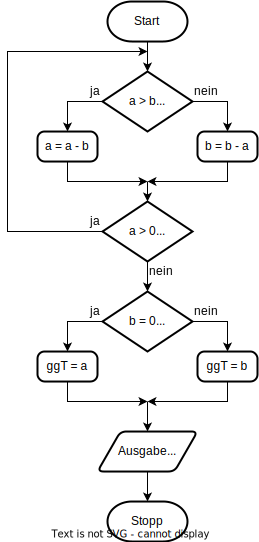
\includegraphics[scale=0.9]{Bilder/Kapitel-1/Abb-1-4.pdf}
    \vspace{\baselineskip} %%% für Druck
    \caption[Der Euklidische Algorithmus als Flussdiagramm]{Ein Flussdiagramm, das den Euklidischen Algorithmus zur Berechnung des größten gemeinsamen Teilers (ggT) zweier positiver Ganzzahlen grafisch darstellt}
    \label{fig:flussdiagramm}
\end{figure}

\pagebreak %%% für Druck

Den gleichen Zweck erfüllten die 1973 vorgestellten 
\marginline{Nassi-Shneiderman-Diagramm}
\textit{Nassi-Shneiderman-Diagramme}, die die Prinzipien der strukturierten Programmierung auf die Ebene des Softwareentwurfs übertrugen und den geplanten Programmablauf in einfachen Diagrammen als Kombinationen aus Sequenzen und Kontrollstrukturen darstellten.

\begin{figure}[h!]
	\centering
	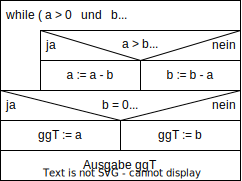
\includegraphics[scale=1.1]{Bilder/Kapitel-1/Abb-1-5.pdf}
	\caption{Der Euklidische Algorithmus als Nassi-Shneiderman-Diagramm}
	\label{fig:nassi_shneiderman_diagramm}
\end{figure}

1977 stellte Douglas Ross, auch ein Teilnehmer der 1968er-Konferenz, die \textit{\mbox{Structured} Analysis and Design Technique} (SADT) \marginline{SADT}
für den Entwurf von Softwaresystemen vor. SADT bildet die Funktionen der (zukünftigen) Software in Form einfacher hierarchischer Diagramme mit Angabe von Eingabe (engl. Input) und Ausgabe (engl. Output) sowie weiteren Informationen (\zb benötigte Ressourcen, äußere Einflüsse) ab. Die Diagramme können sowohl während der Anforderungsanalyse (\zb als Kommunikationsmittel mit dem Auftraggeber über die benötigten Funktionalitäten) als auch in der Entwurfsphase (\zb zur Aufteilung des Systems in Module) verwendet werden. Parallel dazu entwickelten Edward Yourdon und Larry Constantine seit Mitte der 1970er Jahre die Entwurfsmethode \textit{structured design} (SD). \marginline{SD, SA}
Sie selber und auch verschiedene andere Autorinnen und Autoren stellten in den Folgejahren sowohl weitere Varianten dieser Methode vor als auch mit \textit{structured analysis} (SA) Methoden für den Bereich der Anforderungsanalyse. 
 
Den Spezifikations- und Entwurfsmethoden der 1970er Jahre ist gemeinsam, dass die Funktionalitäten der Software nicht als Code einer konkreten Programmier\-sprache, sondern abstrakt als Pseudocode oder durch grafische Notationen (Diagramme) dargestellt werden. Dies führte dazu, dass ungenügend spezifizierte Anforderungen oder Schwachstellen in der Struktur der zukünftigen Software schon vor der Implementierung entdeckt werden konnten -- aber natürlich nicht zwangsläufig immer wurden. Die eigentliche Programmcodeerstellung konnte so systematischer ablaufen und wurde zudem besser planbar, da im Idealfall durch die vorgeschalteten Analyse- und Entwurfsprozesse die später zu implementierenden Funktionen schon feststanden. Die Übertragung der \textbf{Programmier}methoden der 1960er Jahre auf die höhere Abstraktionsebene von \textbf{Spezifikations-} und \textbf{Entwurfs}methoden der 1970er Jahre brachte die Professionalisierung der Softwareentwicklung einen großen Schritt voran.

\sttpDefinitionskasten{\sttpDefinitionskastenSkalierungsfaktor}{Implementierung}{Prozess der Programmcodeerstellung eines Softwareprodukts auf Basis einer in Nicht-Code formulierten Vorlage, wie zum Beispiel ein mathematisch oder allgemeinsprachlich definierter Algorithmus oder ein grafisch oder textuell beschriebener Softwareentwurf.}{In einer zweiten Bedeutung wird mit dem Begriff Implementierung (\textbf{die} Implementierung) häufig auch das Ergebnis der Implementierung, also der entstandene Programmcode bezeichnet. Im Rahmen dieses Textes verwenden wir den Begriff Implementierung in Abgrenzung zu den anderen Prozessen des Softwareengineering (\zb Prozess der Anforderungsermittlung) in seiner ersten Bedeutung.}

\minisec{Entwicklungen der 1980er Jahre}

Mit der Verbreitung der PC (Personal Computer) seit Anfang der 1980er Jahre nahm die Bedeutung von Softwareprodukten noch einmal stark zu. Die Softwarehersteller richteten ihren Blick jetzt auf den gesamten Lebenszyklus ihrer Produkte, von der Erfassung der (vermuteten) Kundenwünsche, über den Softwareentwurf, bis zu Implementierung und Test der Software, und noch weiter zur Wartung und Weiterentwicklung der Softwareprodukte. Gleichzeitig nahm die Anzahl der Entwicklungswerkzeuge für die Softwareentwicklung beständig zu. Schon seit Ende der 1960er Jahre waren im Zuge der strukturierten Programmierung erste Werkzeuge entstanden, die die Programmierer dabei unterstützen sollten, bei der Implementierung die Prinzipien dieser Programmiermethode anzuwenden. Aus heutiger Sicht kann man diese Werkzeuge als die ersten, noch sehr einfachen, \textit{CASE Tools} \marginline{CASE Tools}
(Computer-Aided Software Engineering Tools) bezeichnen. Die bisherigen Werkzeuge zur Unterstützung der Implementierungsarbeiten wurden jetzt in den 1980er Jahren durch solche ergänzt, die Aspekte der Anforderung und des Entwurfs unterstützten. Zudem entstanden die ersten Werkzeuge zum automatisierten Testen von Programmcode sowie Werkzeuge und Hilfen für das Projektmanagement von Softwareentwicklungsprojekten.

Schon seit den 1970er Jahre hatten die Softwarehersteller den Blick auch auf die organisatorisch geprägten Aktivitäten des Softwareentwicklungsprozesses gerichtet. So wurden Konzepte und Techniken der Planung, der Kostenabschätzung, der Steuerung und des Controllings aus dem klassischen Projektmanagement (und zunehmend auch deren Werkzeuge) für die Softwareentwicklung adaptiert. Je komplexer die Softwareentwicklungsprojekte wurden und je mehr Personen an der Erstellung einer Software beteiligt waren, desto stärker versuchte man auch, (gut funktionierende) Arbeitsprozesse auf spätere Projekte zu übertragen. Mit dem Wasserfallmodell und dem Spiralmodell verbreiteten sich so seit Mitte der 1980er Jahre die ersten 
\sttpkapitelverweis{Vorgehens\-modelle}{Kap.~\ref{sec:Kap-2}}
\textit{Vor\-gehens\-modelle} der Softwareentwicklung. Vorgehensmodelle organisieren die Tätigkeiten der Softwareentwicklung in logische Abschnitte und definieren die Übergänge zwischen diesen Abschnitten. Die ersten Vorgehensmodelle waren Phasenmodelle, in denen die Prozesse des Softwareengineering, wie zum Beispiel Anforderungen ermitteln, Softwareentwurf festlegen etc., anhand einer Zeitachse in aufeinanderfolgende Phasen eingeteilt wurden. Spätere Vorgehensmodelle sahen parallele Phasen oder wiederholte zyklische Abläufe der Prozesse vor. Heute werden verschiedene Arten von Vorgehensmodellen in der Softwareentwicklung eingesetzt. 

\minisec{Objektorientiertes Softwareengineering}

Auf der Implementierungsebene sind die späten 1980er Jahre durch das Aufkommen der \textit{objektorientierten Programmierung} geprägt. 
Erste objektorientierte Sprachen hatte es schon seit den 1960er (Simula-67) und 1970er (Smalltalk) Jahren gegeben, aber erst mit der Entwicklung von C$++$ und Objective-C hielten die Prinzipien der objektorientierten Programmierung wirklich Einzug in die Implementierung. Die heute weit verbreitete objektorientierte Sprache Java folgte Mitte der 1990er Jahren und trug viel dazu bei, dass sich die objektorientierte Programmierung so stark durchsetzte. Modularisierung, Geheimnisprinzip und vor allem Wiederverwendung von Programmkomponenten – ein schon auf der 1968er-Konferenz angesprochenes, aber damals kaum beachtetes Thema – sind wichtige Elemente dieses Programmierparadigmas. 

Mit der objektorientierten Programmierung erhielt auch der Bereich der Softwaretests 
%\sttpgls{Softwaretests}
einen höheren Stellenwert. Programmcode, der (evtl. auch vielfach und in verschiedenen Softwareprodukten) wiederverwendet werden soll, stellt höhere Ansprüche an die Qualität des Testprozesses. Aufgrund der starken Modularisierung ist das Testen zudem aufwändig, da sowohl die einzelnen Module als auch das Zusammenspiel der Module getestet werden müssen. Gleichzeitig verringern die Kapselung 
%\sttpgls{Kapselung}
und die definierten Schnittstellen der Module aber die Komplexität der einzelnen Tests und bieten die Möglichkeit, (Teile der) Tests zu automatisieren. 

Wie schon bei der strukturierten Programmierung folgten auf die objektorientierten \textbf{Programmier}methoden entsprechende objektorientierte \textbf{Entwurfs}methoden. Diese unterschieden sich teilweise sehr: Sie waren eng auf eine bestimmte Programmiersprache ausgerichtet, oder bezogen sich nur auf bestimmte Anwendungsgebiete, oder (zurück zu den Anfängen) waren nur für bestimmte Typen von Hardware gedacht. Allen Entwurfsmethoden war aber wieder gemeinsam, dass sie nicht mit Hilfe von Programmcode, sondern abstrakter kommuniziert wurden – im überwiegenden Fall durch Diagramme, teilweise ergänzt um formale textuelle Spezifikationen. Parallel zu den Entwurfsmethoden entwickelten sich Werkzeuge für die Unterstützung des objektorientierten Entwurfs- und Implementierungsprozesses. 

Bei aller Unterschiedlichkeit der objektorientierten Entwurfsmethoden im Detail bauten sie überwiegend auf der Idee auf, zu Beginn eines Softwareentwicklungsprojekts ein sogenanntes \textit{Domänenmodell} 
\marginline{Domänenmodell}
%\sttpkapitelverweis{Domänenmodell}{Kap.~\ref{sec:Kap-3.2.3}}
zu erstellen. Je nach Entwurfsmethode setzte sich dieses aus unterschiedlich vielen Diagrammen und textuellen Spezifikationen zusammen. Im Domänenmodell werden die für die zu entwickelnde Software relevanten Objekte des relevanten fachlichen Bereichs (die sogenannte Domäne), ihre Beziehungen zueinander sowie relevante Prozesse oder Aktivitäten der Domäne in einer auch für Nicht-Programmierer verständlichen Weise modelliert. Das Domänenmodell sollte im Laufe des Softwareentwicklungsprozesses schrittweise in immer detailliertere und in der Darstellungsform immer stärker auf die Implementierung ausgerichtete Modelle transformiert werden. Am Ende des Wegs sollte ein Modell stehen, das sich nach festen Regeln (und idealerweise sogar  automatisiert) in Programmcode umsetzen lässt. 

Die Vielfalt der objektorientierten Entwurfsmethoden erschwerte jedoch die Entwicklung von CASE Tools und die Kommunikation zwischen verschiedenen Softwareentwicklungsprojekten. Um eine vereinheitlichte Notation für die Spezifikation und den Entwurf von Softwaresystemen zu schaffen, arbeitete man in den 1990er Jahren – auf Basis der zu dieser Zeit verbreitetsten objektorientierten Notationen – an der Entwicklung der \textit{Unified Modeling Language (UML)}.
\marginline{UML} 
%\sttpkapitelverweis{UML}{Kap.~\ref{sec:Kap-3.2.2}}
Die Version 1.0 der UML wurde 1997 veröffentlicht. Seitdem hat sie zahlreiche kleinere Änderungen und Ergänzungen, aber auch umfassende Neustrukturierungen erfahren. Heute aktuell ist die Version 2.5.1, die Ende 2017 veröffentlicht wurde. Die UML stellt verschiedene Diagrammarten zur Verfügung, mit denen sich sowohl die Domäne selber als auch statische und dynamische Aspekte des zu entwickelnden Softwareprodukts modellieren lassen. Sie zeichnet sich dadurch aus, dass sie für unterschiedliche Domänen eingesetzt werden kann und (relativ) unabhängig ist von der Wahl des Vorgehensmodells für den Softwareentwicklungsprozess und von der konkreten objektorientierten Programmiersprache der Implementierung. Auf der UML bauen zahlreiche Entwicklungswerkzeuge auf. Das Spektrum reicht von Tools, die bei der Erstellung von UML-Diagrammen unterstützen bis zu solchen, die auf Grundlage von UML-Diagrammen Quellcode bestimmter Programmiersprachen erzeugen.

\minisec{Softwareengineering seit den 1990er Jahren}

Auf der Implementierungsebene entwickelten sich in den 1990er Jahren vermehrt Skriptsprachen. \marginline{Skriptsprachen}
Eine Skriptsprache ist eine Programmiersprache, die über einen Interpreter ausgeführt wird und nicht wie klassische höhere Programmiersprachen compiliert wird. Die frühen Skriptsprachen der 1970er und 1980er Jahre wurden meist nur für kleinere Automatisierungen (\zb einfache Shell- oder Batch-Skripte) verwendet, während Skriptsprachen wie Perl (1987), Python (1991) oder PHP (1995) auch für komplexere Aufgaben eingesetzt werden konnten. Die heute bekannteste Skriptsprache ist JavaScript, deren Version 1.0 im Jahr 1996 eingeführt wurde. Der verstärkte Einsatz von Skriptsprachen seit den 1990er Jahren ist eng verbunden mit der Einführung des World Wide Web (WWW) im Jahr 1991. Skriptsprachen wurden zunächst im WWW nur dafür verwendet dynamische Seiteninhalte in statische HTML-Seiten einzubinden, heute mittlerweile aber überwiegend zur Erstellung kompletter Webanwendungen. 

Das Aufkommen von Internet und WWW führte in den darauffolgenden Jahren und Jahrzehnten auch zu neuen Softwarekonzepten und -architekturen (\zb Client-Server Architekturen, Cloud Computing, Webservices, Software as a Service). Aus Soft\-ware\-engi\-neer\-ing-Sicht bedeutet das vor allem neue Herausforderungen 
\linebreak %%% für Druck
im Bereich Dezentralisierung (verteilte Software) und stark gestiegene Ansprüche im Bereich Wiederverwendung von Komponenten und Programmen. Mit der zunehmenden Verbreitung und Nutzung von anerkannten Entwurfsprinzipien, Entwurfs- und Architekturmustern sowie der stetigen Entwicklung und Verbesserung von 
\linebreak %%% für Druck
Bibliotheken und Frameworks hielt zudem eine ganz neue Ebene von Standardisierung und Wiederverwendbarkeit, aber auch von Abstraktion, Einzug ins Softwareengineering. 

Architektur- und Entwurfsmuster 
\marginline{Muster, Bibliotheken, Frameworks} 
sind abstrakt beschriebene Schablonen bewährter Lösungen für wiederkehrende und gleichartige Probleme, an denen man sich bei der Entwicklung seines eigenen Softwareprodukts orientieren kann. Bibliotheken bestehen aus Sammlungen mit Programmcodekomponenten, die nützliche und allgemeine Funktionalitäten zur Verfügung stellen, die aus dem eigenen Programmcode heraus aufgerufen werden können. Diese Funktionalitäten müssen Entwickler daher in ihrem eigenen Softwareprojekt nicht mehr selber programmieren, sondern nutzen die von anderen dafür erstellten Operationen. Frameworks gehen auf diesem Weg der Wiederverwendung noch einen Schritt weiter. Ein Framework liefert bereits das komplette Grundgerüst für ein Softwareprogramm. Die Entwickler müssen innerhalb dieses Grundgerüsts dann nur noch die Aspekte programmieren, die spezifisch für ihre Software sind, alles andere wird übernommen. Alle diese Konzepte fielen nicht in den 1990er Jahren plötzlich vom Himmel; viele Ursprünge, Vorarbeiten oder mindestens Ideen kann man bereits in den 1970er und 1980er Jahren finden. Erst jetzt setzte sich deren Nutzung aber verbreitet durch. Heute ist kaum ein komplexeres Softwareentwicklungsprojekt denkbar, das nicht in irgendeiner Weise auf Mustern, Bibliotheken oder Frameworks -- in der Regel sogar auf Kombinationen davon -- aufbaut.

\minisec{Weiterentwicklung und Standardisierung}

\sttpAutorenkasten{Grady Booch}{1955}{}{
	\vspace{4mm} %%% für Druck
	US-amerikanischer Informatiker. Entwickelte zusammen mit Ivar Jacobson und James Rumbaugh die UML und wurde dafür mit dem Computer Pioneer Award ausgezeichnet. Arbeitete viele Jahre bei Rational Software und war dort maßgeblich an der Entwicklung des Vorgehensmodells Rational Unified Process beteiligt.
	\vspace{4mm} %%% für Druck
}
{Bilder/Autoren/booch.jpg}{2013}{vonguard, \href{https://creativecommons.org/licenses/by-sa/2.0}{CC BY-SA 2.0}, via \href{https://commons.wikimedia.org/wiki/File:Grady_Booch,_CHM_2011_2_cropped.jpg}{Wikimedia Commons}}

Zum 50jährigen Jubiläum \marginline{Software\-engineering entwickelt sich stetig weiter} des Softwareengineering 2018 verfasste Grady Booch – einer der Pioniere der objektorientierten Softwareentwicklung und maßgeblich an der Entstehung der UML beteiligt – einen Überblicksartikel zur Geschichte des Softwareengineering \cite{boo18}. 
In diesem vertritt er die These, dass Softwareengineering über die Jahrzehnte immer auch in Reaktion auf äußere Zwänge gereift sei. Jede Zeitperiode der letzten fünfzig Jahre stellte anhand von technologischen (\zb verfügbare Hardware, Grad der Vernetzung von Computern), aber auch gesellschaftspolitischen Gegebenheiten (\zb Kalter Krieg, Globalisierung, Wandel der Arbeitswelt) ihre eigenen Anforderungen an Softwaresysteme und erzeugte so (explizit oder implizit) Druck auf das Feld des Softwareengineering, sich entsprechend weiterzuentwickeln. Durch die stetigen technologischen Fortschritte (Weiterentwicklung von Smart\-phones, Tablets etc., Internet of Things) entstanden und entstehen neue Arten von Softwaresystemen und damit wieder neue Herausforderungen für das Softwareengineering. Seit dem Aufkommen agiler Vorgehensmodelle verändern sich darüber hinaus auch Arbeitsprozesse in der Planung und organisatorischen Durchführung von Softwareprojekten.

Ob Softwareengineering eine (wissenschaftliche) Ingenieurdisziplin ist, oder immer noch auf dem Weg dorthin ist sich zu einer zu entwickeln, oder doch \textbf{nur} eine Sammlung von Best Practice Techniken darstellt, oder irgendetwas dazwischen ist, ist eine seit den Anfängen des Softwareengineering wiederholt geführte, kontroverse Diskussion.\footnote{Zusammenfassende Überblicke zu dieser Diskussion finden sich insbesondere bei \cite{dia14}, \cite{mah04}, \cite{gri11}. Wer sich noch intensiver mit dem Thema Softwareengineering als Disziplin befassen möchte, sei zusätzlich auf \cite{sei14} und \cite{wan00} verwiesen.} 
In jedem Fall haben sich über die Jahre verschiedene Merkmale einer Disziplin, wie (Sektionen von) Fachgesellschaften und Berufsverbänden, Gremien, Fachzeitschriften, Curricula, Handbücher und Standards für den Bereich des Softwareengineering herausgebildet. 

\phantomsection
\label{text:Sevocab}
Im Jahr 1983 veröffentlichte das Institute of Electrical and Electronics Engineers (IEEE, \href{https://www.ieee.org/}{www.ieee.org})\footnote{Das IEEE betreibt eine eigene Online-Bibliothek, in der die Artikel der eigenen Fachzeitschriften, Konferenzpublikationen und Standardisierungsdokumente gelistet sind (\href{https://ieeexplore.ieee.org}{https:
		\linebreak %%% für Druck
		//ieeexplore.ieee.org}). Aus dem Netz der FernUniversität besteht kostenloser Zugriff auf die Volltextversionen vieler gelisteter Einträge.} -- ein seit 1963 existierender weltweiter Berufsverband von Ingenieuren, der auch als Standardisierungsgremium agiert -- zum ersten Mal ein Glossar für den Bereich des Softwareengineering. Auf diesem Standard und seiner Nachfolgeversion von 1990 aufbauend entstand in gemeinsamer Arbeit zwischen IEEE und ISO/IEC (Normungsinstitutionen) in den 2000er Jahren die
\marginline{SEVOCAB} 
\textit{SEVOCAB}-Datenbank, mit dem Ziel, in der Profession eine standardisierte Terminologie, ein gemeinsames Begriffs\textbf{verständnis} und eine einheitliche Begriffs\textbf{verwendung} zu etablieren. SEVOCAB steht für „systems and software engineering vocabulary“. Wie der Name schon sagt, finden sich in SEVOCAB Begriffserläuterungen für Begriffe aus dem Bereich des Softwareengineering und des Systems Engineering.\footnote{Systems Engineering beschäftigt sich mit dem gesamten Lebenszyklus und allen Aspekten komplexer technischer Systeme (Hardware und Software, Verfahren und Prozesse, Einbettung in das Anwendungsumfeld).} Die in SEVOCAB enthaltenen Definitionen wurden größtenteils nicht neu entwickelt, sondern aus etablierten Normen und Standards verschiedener Standardisierungs\-gremien dieses Bereichs übernommen. Dadurch finden sich in SEVOCAB auch mehrere, gleichwertig nebeneinander stehende, unterschiedliche Definitionen einzelner Begriffe, jeweils mit Verweis auf den zugrundeliegenden Standard. Eigene Defini\-tionen nimmt SEVOCAB nur an Stellen vor, an denen Bedeutungen aus verschiedenen Standards zu widersprüchlich sind. Neue Entwicklungen im Bereich Systems Engineering und Softwareengineering werden berücksichtigt, indem Definitionen aus abgelösten Standards entfernt und die der neuen Standards hinzugefügt werden. 

\sttpHinweiskasten{1.0}{abgelöste Standards}{Standards, die nicht mehr aktuell sind, werden von den jeweiligen Standardisierungsgremien als „withdrawn“ (zurückgezogen) oder „superseded“ (ersetzt, abgelöst) markiert, um Nutzern zu sig\-na\-li\-sie\-ren, welche Standards noch Gültigkeit haben und welche nicht.}

In regelmäßigen zeitlichen Abständen wird die zum jeweiligen Zeitpunkt bestehende Datenbasis von SEVOCAB als ISO/IEC Norm veröffentlicht. Die online frei verfügbare SEVOCAB-Datenbank (\href{http://www.computer.org/sevocab}{www.computer.org/sevocab}) wird kontinuierlich erweitert, ist in der Regel also aktueller als die letzte veröffentlichte Norm, besitzt nur nicht deren rechtlich akzeptierten Status.

\phantomsection
\label{text:SWEBOK}
Aufbauend auf vorhandenen Standards 
\marginline{SWEBOK - Kompendium des Software\-engineering}
arbeiteten internationale Softwareingenieure unter Führung des IEEE seit Ende der 1990er Jahre daran, ein Kompendium des Softwareengineering zu erstellen. Ziel ist es, den Kern des allgemein akzeptierten, in der Praxis verwendeten und als wesentlich identifizierten Wissens („core body of knowledge“) für das Berufsfeld des Softwareengineering – auch im Hinblick auf Ausbildung und Fortbildung – zu strukturieren und zugänglich zu machen. Ausdrücklich nicht berücksichtigt werden sollten das Expertenwissen kleinerer Gruppen sowie laufende Forschungsfragestellungen. Ergebnis des (aufgrund intensiver Reviewverfahren) mehrjährigen Prozesses ist der 2004 erstmals erschienene „Guide to the Software Engineering Body of Knowledge“ (\textit{SWEBOK}). 
%\sttpMarginPicture{Bilder/Kapitel-1/Buchcover-SWEBOK.jpg}
Die aktuelle Version SWEBOK V3.0 aus dem Jahr 2014 \cite{swe14} kann nach einer Registrierung kostenlos von der Website der IEEE Computer Society heruntergeladen werden (\href{http://www.computer.org/web/swebok}{www.computer.org/web/swebok}). Aktuell wird an der Version 4.0 gearbeitet. 

SWEBOK teilt das Themenfeld Softwareengineering in fünfzehn Wissensgebiete („knowledge areas“) ein. Dazu gehören neben konkreten Prozessen der Softwareentwicklung wie Anforderungsanalyse und Softwareentwurf auch übergreifende Themen wie Soft\-ware\-qua\-li\-tät sowie notwendige Basis-Wissensgebiete wie Mathematische Grundlagen des Softwareengineering. 

Jedes Wissensgebiet wird kompakt auf fünfzehn bis zwanzig Seiten dargestellt. Dabei geht es weniger darum, konkretes Faktenwissen zu vermitteln, sondern darum, auf einer höheren Abstraktionsebene (hierarchische) Beziehungen, Überschneidungen und Abgrenzungen zwischen einzelnen Themen des Softwareengineering darzustellen. So beschäftigt sich zum Beispiel das Unterkapitel zu Vorgehensmodellen inhaltlich gar nicht mit den zwei wichtigen Vertretern Wasserfallmodell und Scrum, sondern erläutert, welche Kategorien von Vorgehensmodellen im Softwareengineering eingesetzt werden und nach welchen Kriterien sie sich voneinander abgrenzen lassen. 

Die Autorinnen und Autoren von SWEBOK haben zudem sehr darauf geachtet, jedes Kapitel – ein Kapitel entspricht einem Wissensgebiet – einheitlich zu gliedern und Beziehungen zwischen den Wissensgebieten deutlich herauszustellen. Die für SWEBOK verwendete Art der Strukturierung hat den Vorteil, dass das präsentierte Wissen weniger schnell veraltet. Zudem bietet sie einen stark analytischen Zugang zum Feld des Softwareengineering. Für Anfänger im Softwareengineering nachteilig kann aber der hohe Abstraktionsgrad der Texte sein. Daher werden für die fakten\-orien\-tier\-tere Beschäftigung mit den Themen in allen Unterkapiteln Verweise auf konkrete Kapitel und sogar einzelne Seiten von Lehrbüchern angegeben, die die Autorinnen und Autoren des SWEBOK als Standardliteratur zum entsprechenden Gebiet identifiziert haben. 

% 1.2
\clearpage
\section{Softwareengineering heute}
\label{sec:Kap-1.2}
% Für diesen Abschnitt ist kein Text vorgesehen.
\subsection{Was ist Softwareengineering?}
\label{sec:Kap-1.2.1}

Softwareengineering wurde erstmalig bedeutsam, als Software breitentauglicher (Einsatz auch außerhalb von Forschungseinrichtungen) werden sollte und gleichzeitig die Einsatzfelder von Software zu kritisch waren (\zb Verteidigungssysteme, medizinische Geräte), als dass man „ungeplant“ hätte entwickeln können. Aus den bisherigen Darstellungen sollte deutlich geworden sein, dass es im Laufe der letzten Jahrzehnte sich verändernde, ergänzende, aber teilweise auch konkurrierende Vorstellungen gab, welche Aspekte Softwareengineering beinhalten und in welche Richtung es sich weiterentwickeln soll. Wenn man heute in Lehrbüchern nach Definitionen zum Softwareengineering sucht, findet man -- trotz Standardisierungsbemühungen wie den Arbeiten an SWEBOK -- immer noch viele verschiedene Vorschläge. Zum einen unterscheiden sie sich darin, welche Prozesse aus dem Bereich der Erstellung von Software dem Softwareengineering zugerechnet werden und welche nicht: Gehören beispielsweise die Kostenkalkulation des Softwareprojekts, die Zusammenstellung des Entwicklerteams oder die Wahl des Vorgehensmodells schon in den Bereich Softwareengineering oder beginnt Softwareengineering erst \textbf{danach}? Wann endet Softwareengineering: Inwiefern gehören Wartung, Weiterentwicklung, aber auch Vertrieb der Software dazu? Zum anderen gehen die Meinungen, inwieweit Softwareengineering eine (echte) ingenieurwissenschaftliche Disziplin ist, auch heute noch auseinander (dasselbe gilt im Übrigen auch für die gesamte Informatik). Die Gründe für die unterschiedlichen Vorstellungen über das Gebiet Softwareengineering sind die gleichen wie vor fünfzig Jahren: Menschen mit unterschiedlichen (beruflichen) Hintergründen oder unterschiedlichen aktuellen Arbeitsgebieten definieren Softwareengineering und vor allem auch das Aufgabengebiet von Softwareingenieuren und -ingenieurinnen unterschiedlich.

Nichtsdestotrotz
\marginline{Prinzipien des Ingenieur\-wesens für die Entwicklung von Software nutzen} 
besteht heute Einigkeit darüber, dass Softwareengineering sich dadurch auszeichnet, dass Prinzipien des Ingenieurwesens auf die Entwicklung von Software angewendet werden. Dazu gehören die systematische Entwicklung und Verwendung von Methoden, Standards und Werkzeugen und die Entwicklung von Maßsystemen zur Messung und Qualitätsbeurteilung von Softwareeigenschaften genauso wie die intensive Nutzung von Erfahrungswerten.

Des Weiteren sind folgende Punkte Konsens: 
\begin{itemize}
	\item Softwareengineering ist mehr als nur Programmierung, beinhaltet also noch weitere Prozesse.
	\item Softwareengineering beschäftigt sich mit der \textbf{systematischen} Entwicklung von \textbf{komplexer} Software. Es geht also zum einen darum, geplant zu entwickeln, statt „irgendwie zu programmieren“. Und zum anderen liegt der Fokus auf den größeren, komplexeren Softwaresystemen und nicht auf dem kleinen, einfachen Programm zur automatischen Bewässerung der eigenen Zimmerpflanzen.
	\item Softwareengineering beruht neben theoretischen (mathematischen) Grund\-lagen auch auf heuristischen Techniken und Methoden (Best Practices).
\end{itemize}

\pagebreak %%% für Druck

Der schon erwähnte SEVOCAB-Standard definiert Softwareengineering dementsprechend als: 

\sttpzitat{„systematic
\marginline{Definition\\Software\-engineering} 
application of scientific and technological knowledge, methods, and experience to the design, implementation, testing, and documentation of software.”}{Eintrag „software engineering“ bei \href{http://www.computer.org/sevocab}{www.computer.org/sevocab}}

\vspace{\baselineskip} %%% für Druck

Die SEVOCAB Softwareengineering-Definition stellt die theoretisch fundierten Erkenntnisse und die Erkenntnisse aus praktischen Erfahrungen gleichwertig neben\-einander. Wie Sie im Laufe des Textes noch lesen werden, dominieren aber in manchen Prozessen des Softwareengineering – vor allem in der Anforderungsermittlung und im Entwurf – heute die Best Practice Techniken. Eine theoriegeleitete Beschäftigung mit Softwareengineering existiert nichtsdestotrotz auch heute noch, und dies hat auch eine starke Berechtigung. Einerseits werden hier Grundlagen entwickelt, die in der Zukunft die Softwareentwicklung revolutionieren könnten. Zum Anderen unterscheiden sich Softwaresysteme unter anderem darin, welche Konsequenzen Fehler haben. Stark sicherheitskritische Anwendungen, zum Beispiel in der Raumfahrt oder in der Medizintechnik, erfordern ein weit höheres Maß an Vertrauen in die Korrektheit von Software als andere Anwendungen; hier spielen formale Methoden weiterhin eine große Rolle.

\vspace{\baselineskip} %%% für Druck

\phantomsection
\label{text:theoVertreter}

\sttpKastenBreakable{\textbf{formale Methoden vs. Best Practices}

Schon lange vor der Entstehung von agilen Entwicklungsansätzen, die in den 1990er Jahren eine bis heute bestehende Konfliktlinie zwischen Befürwortern und Gegnern agiler Softwareentwicklung eröffneten (s. Kap.~\ref{sec:Kap-2.3}), existierte im Softwareengineering eine ältere Konfliktlinie zwischen zwei wettstreitenden Fraktionen: diejenigen, die an formale Methoden und Korrektheitsbeweise für Software glaubten, und diejenigen, die all diese mathematisch-logisch orientierten Methoden für nicht praktikabel und viel zu aufwändig hielten. Beide Seiten hielten sich gegenseitig mangelhaftes ingenieurmäßiges Denken vor: Die formale Fraktion verwies auf die formalen Grundlagen in den anderen Ingenieurwissenschaften (\zb Statikberechnungen), die andere Seite verwies auf die Orientierung an Best Pratices und die Notwendigkeit, Methoden für aktuell existierende Probleme und aktuelle Softwareentwicklungsprojekte zu erstellen, statt Grundlagen für irgendeine Zukunft zu legen. Formale Spezifikationen zu Projektbeginn bei der Formulierung von Anforderungen können in diesem Zusammenhang als ein Kompromiss betrachtet werden. Die Vision der formalen Fraktion war und ist, dass Software eigentlich gar nicht mehr (von Menschen) entwickelt werden muss, sondern automatisch aus hinreichend präzisen Anforderungen generiert wird und dann per Konstruktion diese Anforderungen erfüllt (natürlich muss dafür auch diese Generierungssoftware fehlerfrei sein). Mit diesem Ziel wurden und werden eigene Sprachen für die Spezifikation und auch neue Programmiersprachen entwickelt. Man könnte diese Forschungsrichtungen ebenfalls Softwareengineering nennen, tatsächlich verteilen sie sich aber über andere Teildisziplinen der Informatik, und werden auch an der FernUniversität in anderen Modulen gelehrt. Deshalb gehen wir auch in diesem Text den sehr formalen Ansätzen nicht intensiver nach. Bemerkenswert bleibt aber, dass die Ursprünge des Softwareengineering durchaus auch auf eher formalen Ansätzen beruhten und beide genannten Fraktionen anfangs beteiligt waren.}

\vspace{\baselineskip} %%% für Druck

Softwareengineering ist ein Fachgebiet, das sich weiterhin im Wandel befindet. Anhand der Herausforderungen neuer Softwarekonzepte oder neuer Arten von Soft\-ware\-syste\-men entstehen neue, erweiterte oder veränderte Programmiersprachen, Notationen, Vorgehensmodelle, Methoden und Techniken in allen Bereichen des Soft\-ware\-lebens\-zyklus - und das meist außerhalb des wissenschaftlichen Bereichs. Jenseits aller Standardisierungsbemühungen und verschiedener Versuche, der Disziplin ein stärkeres wissenschaftliches Fundament zu geben, wird sich Softwareengineering auch weiterhin in erster Linie dadurch definieren, welche Fähigkeiten ein Soft\-ware\-inge\-nieur in der Praxis benötigt und was er in seiner täglichen Arbeit tut. Die universitäre Lehre (und einen Lerntext zum Thema Softwareengineering) stellt dies vor große Herausforderungen. Wenn wir uns zu sehr auf die neuesten oder aktuell beliebtesten Entwurfsmethoden, Frameworks oder Entwicklungswerkzeuge konzentrieren, könnte das, was wir heute als neueste Errungenschaften lehren, morgen schon wieder veraltet sein. Es könnte sich auf der anderen Seite in der Praxis (noch) nicht durchgesetzt haben bzw. sich nie durchsetzen. Um das beliebte Beispiel der Vorgehensmodelle noch einmal zu bemühen: Wir können sowohl Scrum als auch das Wasserfallmodel vorstellen (und werden das auch tun), aber aus Lehrperspektive wichtiger ist die Vermittlung, was ein Vorgehensmodell auszeichnet, warum man es im Softwareengineering einsetzt und welche Vor- und Nachteile unterschiedliche Kategorien von Vorgehensmodellen haben.

Heute gibt es sehr viele unterschiedliche Arten von Softwaresystemen, für die unterschiedliche Softwareengineering-Techniken erforderlich sind. So werden sich das Softwareengineering für eine stand-alone Fotobearbeitungssoftware, für ein eingebettetes System eines Autos und für eine Webanwendung eines Onlineshops in den eingesetzten Programmiersprachen, Vorgehensmodellen und Entwurfstechniken stark unterscheiden.
\marginline{die grundlegenden Aspekte des Software\-engineering} 
Die unterliegenden Ideen und Konzepte des Softwareengineering lassen sich aber für alle Softwaresysteme anwenden: Für jede industriell gefertigte Software müssen in irgendeiner Art und Weise Anforderungen spezifiziert werden, die in irgendeiner Notation dokumentiert werden müssen. Jede Software durchläuft irgend\-wann einen oder mehrere Entwurfsprozess(e), muss implementiert, verifiziert oder getestet, an die Kunden ausgeliefert und gewartet werden. Und alle diese Aktivitäten müssen innerhalb gegebener Zeit-, Kosten- und Personalbudgets in hoher Qualität erfolgreich abgeschlossen werden. Dementsprechend beschäftigt sich dieser Text schwerpunktmäßig mit den grundlegenden Aspekten des Softwareengineering, die unabhängig von der Art des zu entwickelnden Softwaresystems eine Bedeutung haben.

\clearpage %%% für Druck
\subsection[Rollen, Prozesse, Aktivitäten – Begriffe des Software-\\engineering]{Rollen, Prozesse, Aktivitäten – Begriffe des Softwareengineering}
\label{sec:Kap-1.2.2}

An einem Softwareentwicklungsprojekt sind in der Regel verschiedene Personengruppen beteiligt, die im Englischen und mittlerweile zunehmend häufiger auch in deutschsprachiger Literatur mit dem Begriff \textit{Stakeholder} \marginline{Stakeholder} 
(Interessenvertreter) bezeichnet werden. Zu den Stakeholdern eines Softwareentwicklungsprojekts zählen zum Beispiel Softwareentwickler, Softwarearchitekten, Tester, Qualitätssicherungsexperten, Projektleiter, Domänenexperten, Auftraggeber, (zukünftige) Nutzer. 

Je nach Projektgröße werden unterschiedlich viele Personen am Projekt beteiligt sein. Gerade bei kleineren Projekten muss ein konkretes Teammitglied oft mehrere Aufgaben wahrnehmen, zum Beispiel könnten die Aufgaben der Soft\-ware\-archi\-tektin 
%\sttpgls{Softwarearchitekt}
von einer der Softwareentwicklerinnen mit übernommen werden oder der Auftraggeber gleichzeitig der Domänenexperte 
%\sttpgls{Domaenenexperte}
sein. In großen Projekten könnten mehrere Teammitglieder identische oder ähnliche Aufgabengebiete besitzen oder ein Aufgabengebiet von wechselnden Personen übernommen werden. Wenn man über das Team spricht, das an einem Softwareentwicklungsprojekt beteiligt ist, abstrahiert man daher von konkreten Personen und spricht stattdessen von sogenannten Rollen. Jeder Rolle sind bestimmte Aufgaben zugeordnet. Zudem ist sie mit spezifischen Kenntnissen und Fähigkeiten verknüpft, die benötigt werden, um die der Rolle zugeordneten Aufgaben ausführen zu können. Im konkreten Projekt nimmt jedes Teammitglied eine oder mehrere Rollen ein und führt die der Rolle/den Rollen zugeordneten Tätigkeiten aus.

\sttpDefinitionskasten{\sttpDefinitionskastenSkalierungsfaktor}{Rolle im Softwareentwicklungsprojekt}{Abstrakte Beschreibung einer anonymen Person mit definierten Aufgaben und Befugnissen und entsprechenden Kenntnissen und Fähigkeiten.}{Das Konzept der Rolle ist im Softwareengineering mit mehreren Bedeutungen verbunden. In diesem Zusammenhang geht es um die Beschreibung von Akteuren im Rahmen der Softwareentwicklung.}

Die innerhalb eines Softwareentwicklungsprojekts durchgeführten einzelnen Tätigkeiten (\zb das Lastenheft schreiben, den Testplan erstellen, eine bestimmte Funk\-tion implementieren) kann man verschiedenen großen Bereichen des Soft\-ware\-entwick\-lungs\-prozesses zuordnen, wie zum Beispiel dem Bereich der Implementierung oder dem Bereich des Testens. Diese Teilbereiche des Softwareentwicklungsprozesses bezeichnen wir als \textit{Prozesse}. 

\begin{figure}[h!]
	\centering
	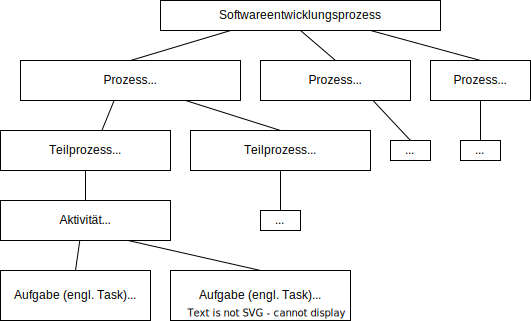
\includegraphics[scale=1.0]{Bilder/Kapitel-1/Abb-1-6.pdf}
	\caption{Zusammenhang zwischen Prozessen, Aktivitäten und Aufgaben}
	\label{fig:prozesse_aktivitaeten_aufgaben}
\end{figure}

Abbildung~\ref{fig:prozesse_aktivitaeten_aufgaben} zeigt den Zusammenhang \marginline{Prozess, Aktivität, Aufgabe} der in diesem Text verwendeten Begriffe: Ein Prozess, wie zum Beispiel der Prozess der Anforderungsermittlung, kann in \mbox{\textit{Teilprozesse}} weiter unterteilt werden. Jeder Teilprozess besteht aus einer Menge von \textit{Aktivitäten}, wie zum Beispiel „Lastenheft erstellen“ oder „Module der Software bestimmen“. Aktivitäten wiederum können in noch kleinere Einheiten, sogenannte \textit{Aufgaben} (engl. Tasks), unterteilt werden, die schlussendlich von Rollen ausgeführt werden. Ein konkreter Softwareentwicklungsprozess ist somit eine Menge aus einzelnen Aktivitäten zusammengesetzter Prozesse. Dabei können sich die Prozesse oder Teilprozesse auch überschneiden, sodass es häufig nicht möglich ist genau zu bestimmen, an welcher Stelle ein Prozess bzw. Teilprozess endet und ein anderer beginnt. Ebenso lässt sich nicht immer eindeutig bestimmen, welchem Teilprozess eine konkrete Aufgabe zugeordnet ist. 

Der Software Engineering Body of Knowledge (SWEBOK) definiert einen ingenieurwissenschaftlichen Prozess als

\sttpzitat{„a set of interrelated activities that transform one or more inputs into outputs while consuming resources to accomplish the transformation“. \cite[8-1]{swe14}}{}

Bezogen auf den Gesamtprozess der Entwicklung eines Softwareprodukts besteht der Input aus der Menge der Anforderungen an die zu erstellende Software und der Output aus dem fertigen Softwareprodukt. Die einzelnen Prozesse innerhalb des Softwareentwicklungsprozesses transformieren unterschiedliche Arten von Inputs in Outputs, wobei die Outputs eines Prozesses oft die Inputs eines oder mehrerer Folgeprozesse sind. So könnte zum Beispiel der Output eines Implementierungsprozesses ein Stück Programmcode sein und Letzteres ein Teil des Inputs für den Prozess des Testens. Bei den verbrauchten Ressourcen für die Erstellung des Softwareprodukts handelt es sich in erster Linie um die Arbeitszeit der an der Entwicklung beteiligten Personen. Ressourcen können aber zusätzlich auch Softwareressourcen (\zb fertige Softwarekomponenten, die in das Produkt eingebunden werden, oder für die Entwicklung verwendete Tools) und Hardwareressourcen (\zb Entwicklungsinfrastruktur) sein. 

\sttpHinweiskasten{1.0}{unterschiedliche Begriffsverwendung}{Beachten Sie, dass Teile der Literatur die großen Bereiche des Software\-entwicklungsprozesses wie Anforderungsermittlung/-analyse, Implementierung oder Testen nicht als \textbf{Prozesse}, sondern schon als \textbf{Aktivitäten} bezeichnen. Für konkrete Tätigkeiten, wie zum Beispiel für die Tätigkeit „das Lastenheft erstellen“ innerhalb der Anforderungs\-ermitt\-lung/-analyse werden dann Begriffe wie Unteraktivitäten oder Sub-Aktivitäten verwendet.}

Bei den angesprochenen Prozessen 
\marginline{Kernprozesse, unterstützende Prozesse}
des Softwareengineering unterscheidet man \textit{Kernprozesse} (engl. primary processes, development processes, implementation processes) von \textit{unterstützenden Prozessen} (engl. support processes). Letztere werden häufig auch als Softwaremanagementprozesse bezeichnet. Seit Mitte der 1980er Jahre besteht relative Einigkeit darüber, welche \textbf{Kernprozesse} dem Softwareengineering zuzurechnen sind, auch wenn die Benennungen, die konkreten Aktivitäten und die Abgrenzungen zwischen den Prozessen je nach Blickwinkel differieren können. Die Kernprozesse des Softwareengineering sind:
\begin{itemize}
	\item die Anforderungsermittlung/-analyse
	\item der Softwareentwurf
	\item die Implementierung
	\item das Testen bzw. allgemeiner die Qualitätssicherung sowie
	\item die Wartung, ggf. ergänzt um die Weiterentwicklung der Software
\end{itemize}

Mittlerweile ist unbestritten, dass neben den Kernprozessen auch Softwaremanagementprozesse Teil des Softwareengineering sind. Welche Managementprozesse dies genau betrifft, variiert aber stark in der Literatur. Der Schwerpunkt unserer Lehrveranstaltung liegt auf den Kernprozessen des Softwareengineering. 

\minisec{Aufbau des Textes}

Lassen Sie uns an dieser Stelle die inhaltliche Ebene kurz verlassen und auf die noch ausstehende Darstellung zum Aufbau des Textes zurückkommen. Kapitel~\ref{sec:Kap-2} in dieser ersten Lektion behandelt das Thema der Vorgehensmodelle und deren Zusammenhang zu den Prozessen des Softwareengineering. Die detaillierte Beschäftigung mit den eben vorgestellten Kernprozessen des Softwareengineering beginnt ab Lektion 4. Zuvor werden sich die Lektionen 2 und 3 allgemeiner mit dem Thema Modellierung beschäftigen, das in allen Prozessen des Softwareengineering eine Rolle spielt. Wie erwähnt legt der Text den Schwerpunkt auf grundlegende Aspekte des Softwareengineering, die weitestgehend unabhängig von der Art des (zu entwickelnden) Softwareprodukts sind. Einige andere Einschränkungen müssen wir aber treffen, um den Umfang im Rahmen zu halten: Die Lehrveranstaltung beschäftigt sich nur mit objektorientierter Softwareentwicklung und aus der Menge der möglichen Notationssprachen wird die Unified Modeling Language (UML) gewählt, die die bei Weitem größte Verbreitung genießt.  

% 1.3
% Kommentierte Literatur beginnt auf neuer Seite
\clearpage
\section{Kommentierte Literatur}
\label{sec:Kap-1.3}

%Bilder/Buchcover/Buchcover_Naur_Randell.png
\sttpKommLitItem{Naur/Randell}{1969}{Software Engineering: Report on a Conference 1968}{nau69}{}{}
{Der Abschlussbericht zur Softwareengineering-Konferenz in Garmisch 1968. Die Diskussionen auf der Konferenz wurden detailliert protokolliert und zu großen Teilen sogar auf Band aufgenommen, sodass der Bericht neben der Zusammenfassung des Dis\-kussions\-verlaufs auch Originalredebeiträge der Teilnehmer aus den Diskussionen darstellen kann. Eine redaktionelle Bearbeitung durch die Herausgeber des Berichts erfolgte dabei nur insofern, dass die Redebeiträge unabhängig von ihrer chronologischen Reihenfolge thematisch zugeordnet sowie inhaltlich passende Passagen aus den auf der Konferenz vorgestellten Working Papers der Darstellung des Dis\-kus\-sions\-verlaufs hinzugefügt wurden. Zur Folgekonferenz in Rom im Jahr 1969 existiert ebenfalls ein Abschlussbericht \cite{bux70}.}

%{Bilder/Buchcover/Buchcover_Laplante.jpg}{S. 1119-1126}
\sttpKommLitItem{Grier}{2011}{Software Engineering: History}{gri11}{}{}
{Sechsseitiger überblicksartiger Artikel zur Geschichte des Softwareengineering aus der Enzyklopädie des Softwareengineering \cite{lap11} unter dem Blickwinkel, durch welche Entwicklungen sich Softwareengineering zu einer eigenen Disziplin entwickelt hat. Die Meilensteine der sehr frühen Jahre werden chronologisch dargestellt. In der Folge beleuchtet der Artikel dann systematisch, welche Entwicklungen seit den 1970er Jahren bis Ende der 1980er Jahre bezüglich der Prozesse Spezifikation, Entwurf, Implementierung, Test und Wartung von Software wichtig waren. Abschließend beschäftigt sich der Artikel mit der Frage, welche der Merkmale einer Disziplin (Fachgesellschaften, Curricula, Handbücher etc.) Softwareengineering in der Gegenwart (2011) aufweist und inwiefern sich Softwareengineering von den klassischen Ingenieurwissenschaften unterscheidet.}

%{Bilder/Buchcover/Buchcover_Gonzalez.jpg}{72-1 bis 72–20}
\sttpKommLitItem{Díaz-Herrera/Freeman}{2014}{Discipline of Software Engineering: An Overview}{dia14}{}{}
{Ein umfangreicher Artikel aus dem Handbuch Computer Science and Software \linebreak %%% für Druck
	Engineering \cite{gon14}, der einen sehr detaillierten Überblick über die wichtigen Entwicklungen im Softwareengineering von den Anfängen bis zur Gegenwart (2014) gibt. Der Artikel verweist dabei auch intensiv auf die historischen Dokumente zur Softwareentwicklung (wie \zb die Arbeiten von Dijkstra und Parnas). Er ist daher sehr gut als Ausgangspunkt geeignet, um sich noch intensiver in die Geschichte des Softwareengineering zu vertiefen. Der Artikel stellt außerdem die Diskussion vor, ob und inwiefern Softwareengineering eine Disziplin ist.}

%Bilder/Buchcover/zeitung.png
\sttpKommLitItem{Booch}{2018}{The History of Software Engineering}{boo18}{}{}
{Inhaltlich sehr dichter (Aufzählung vieler Personen und Ereignisse) siebenseitiger Artikel zum 50jährigen Jubiläum des Softwareengineering über dessen Entwicklung, geschrieben von einem der Pioniere der objektorientierten Softwareentwicklung und der UML. Im Gegensatz zu der anderen hier vorgestellten Literatur beschäftigt sich der Artikel auch mit frühen Ereignissen der Computerhistorie des späten 19. und frühen 20. Jahrhundert (Babbage, ENIAC, Turing etc.). Zudem listet er Errungenschaften des Softwareengineering ab den späten 1990er Jahren auf, was die anderen hier vorgestellten Artikel zur Geschichte des Softwareengineering aufgrund ihrer Fokussierung auf die Disziplinfrage etwas vernachlässigen. Der Fokus des Artikels liegt dabei immer auf der Darstellung von technologischen und gesellschaftspolitischen Gegebenheiten der jeweiligen Jahrzehnte und deren Auswirkungen auf die Ausrichtung des Softwareengineering.}

%Bilder/Buchcover/zeitung.png
\sttpKommLitItem{del Águila/Palma/Túnez}{2014}{Milestones in Software Engineering and Know\-ledge Engineering History: A Comparative Review}{del14}{}{}
{Der Zeitschriftenartikel vergleicht die Meilensteine in der Entwicklung des Softwareengineering mit denen in der Entwicklung des Knowledge Engineering\footnote{in Deutsch: Wissensmodellierung. Das Themenfeld Knowledge Engineering in der Informatik beschäftigt sich mit der Erforschung und Entwicklung wissensbasierter Systeme. Es ist ein Teilgebiet des Bereichs künstliche Intelligenz.}. Für die Darstellung der Entwicklungen im Softwareengineering verwenden die Autorinnen und Autoren eine Kategorisierung von \cite{end97} aus dem Jahr 1996, die die Geschichte des Softwareengineering in wenige große zeitliche Phasen einteilt, und erweitern diese bis in die Gegenwart (2014). Dadurch zeigt der Artikel stärker als die bisher erwähnte Literatur die größeren Linien in der Geschichte des Softwareengineering, ist gleichzeitig aber auch deutlich weniger detailliert bezüglich der einzelnen Errungenschaften. Der eigentliche Fokus des Artikels liegt auf der Frage, wie Softwareengineering und Knowledge Engineering voneinander lernen und sich weiterentwickeln können.}

%Bilder/Buchcover/zeitung.png
\sttpKommLitItem{Mahoney}{2004}{Finding a History for Software Engineering}{mah04}{}{}
{Ein etwas anderer Ansatz die Entwicklung des Softwareengineering darzustellen. Der Wissenschaftshistoriker Michael Mahoney beleuchtet in seinem Zeitschriftenartikel die akademische und berufliche Sozialisation der Teilnehmer der 1968er-Konferenz, um zu erklären, warum es auf der Konferenz und auch bis in die Gegenwart (2004) so unterschiedliche Ansichten darüber gibt, in welche Richtung sich Softwareengineering entwickeln soll. Er identifiziert drei Gruppen [s. S.~\pageref{text:Mahoney}]. Im Rahmen der Vorstellung dieser drei Gruppen führt der Artikel wichtige Meilensteine der Entwicklung des Softwareengineering auf.}

%Bilder/Buchcover/Buchcover_Tanenbaum_Austin.jpg
\sttpKommLitItem{Tanenbaum/Austin}{2014}{Rechnerarchitektur: Von der digitalen Logik zum \\ %%% für Druck
	Parallelrechner}{tan14}{}{}
{Ein auch für Anfänger sehr gut verständliches Lehrbuch mit umfangreichen Informationen zu den verschiedenen Computergenerationen, zu Compilern, Assemblern und vielen weiteren hardwarenahen Themen.}

%Bilder/Buchcover/zeitung.png
\sttpKommLitItem{Wirth}{2008}{A Brief History of Software Engineering}{wir08}{}{}
{Ein auf sieben Seiten sehr persönlich geprägter Blick auf die Geschichte des Softwareengineering von Niklaus Wirth. Der Artikel beschäftigt sich schwerpunktmäßig mit der Implementierungsebene und den dortigen Entwicklungen der 1960er bis 1980er Jahre.}

%Bilder/Buchcover/Buchcover_Sommerville.jpg
\sttpKommLitItem{Sommerville}{2018}{Software Engineering}{som18}{}{}
{Die Entwicklung des Softwareengineering ist in der neuesten Auflage auf die Web\-site zum Buch (\href{https://software-engineering-book.com/web/history/}{https://software-engineering-book.com/web/history/}) ausgelagert worden und wird nur sehr knapp dargestellt. Im ersten Kapitel des Buchs beschäftigt sich der Autor unter anderem mit den heute existierenden unterschiedlichen Arten von Softwaresystemen und der Frage, warum die Fundamente des Softwareengineering trotzdem für alle gelten (und gelehrt werden können). Die verschiedenen informationstechnischen und organisatorischen Prozesse des Softwareengineering werden ausführlich und jeweils mit Bezug zu vier Fallstudien, die im ersten Kapitel des Buchs vorgestellt werden, behandelt.}

%Bilder/Buchcover/Buchcover_SWEBOK.jpg
\phantomsection
\label{sec:Kap-1.4:Bourque}
\sttpKommLitItem{Bourque/Fairley (Hrsg.).}{2014}{SWEBOK V3.0}{swe14}{}{}
{Kompendium des Softwareengineering [s. {S.~\pageref{text:SWEBOK}}], unter \href{http://www.computer.org/web/swebok}{www.computer.org/web/ \linebreak %% für Druck
		swebok} als PDF verfügbar. Kapitel 8 des SWEBOK beschäftigt sich umfassend mit Soft\-wareen\-gi\-nee\-ring-Prozessen und ist Grundlage für die hier in Abschnitt~\ref{sec:Kap-1.2} dargestellten Inhalte.}

%{Bilder/Buchcover/Buchcover_Laplante.jpg}{S. 684–703}
\phantomsection
\label{sec:Kap-1.4:Shafer}
\sttpKommLitItem{Shafer}{2011}{Process}{sha11}{}{}
{Der Artikel aus der Enzyklopädie des Softwareengineering \cite{lap11} bietet eine sehr umfassende Darstellung des Prozessbegriffs im Bereich Softwareengineering. Neben der Darstellung, wie sich ein Prozess des Softwareengineering definiert, was er be\-inhal\-tet und wie er sich verbessern lässt, behandelt der Artikel auch den Zusammenhang zwischen den Softwareengineeringprozessen und Vorgehensmodellen, mit denen wir uns in Kapitel~\ref{sec:Kap-2} dieser Lektion beschäftigen. Der Artikel von Shafer stellt zudem SWEBOK (in der Version von 2004) und andere internationale Standards vor, die Softwareengineering-Prozesse behandeln.}

%Bilder/Buchcover/Buchcover_Dumke.jpg
\sttpKommLitItem{Dumke}{2003}{Software Engineering}{dum03}{}{}
{Im Unterschied zu den meisten anderen Büchern zum Thema wird Softwareengineering hier aus einer Ingenieurperspektive statt aus einer Informatikerperspektive betrachtet. Deutlich stärker als in anderer Literatur richtet sich der Blickwinkel daher auf die Frage, was eigentlich das ingenieurmäßige am Softwareengineering ist. Für das Themenfeld dieses ersten Kapitels des Textes relevant sind vor allem die Abschnitte 1.1 und 1.2 des Buchs. In Abschnitt 1.1 stellt der Autor grundlegende Begriffe des Softwareengineering vor – in ausführlicherem Umfang, als wir es im Rahmen dieses Kapitels getan haben. In Abschnitt 1.2 werden auf knapp 80 Seiten die Kernprozesse des Softwareengineering anhand von fünf kleinen Softwareproduktbeispielen beschrieben.}

